\documentclass[11pt]{article}

\usepackage{latexsym}
\usepackage{amsmath}
\usepackage{amssymb}
\usepackage{graphicx}
\usepackage{theorem}
\usepackage{enumerate}
\usepackage{tikz}
\usepackage{circuitikz}
\usepackage{hyperref}
\usepackage{changepage} 

% \newtheorem{problem}{Problem}
\newcounter{problem}
\newenvironment{problem}[2][]{\refstepcounter{problem}\par\medskip
   \noindent \textbf{Problem \theproblem~(#2 points):}}{\vspace{1cm}}
\newcounter{subproblem}[problem]
\renewcommand{\thesubproblem}{\roman{subproblem}}
\newenvironment{subproblem}[2][]{\refstepcounter{subproblem}\par\medskip
\begin{adjustwidth}{\parindent}{}
   \textbf{\thesubproblem. (#2 points):}}{\end{adjustwidth}}
\begin{document}

\title{DS-GA 1018: Homework 1}
\author{Due Friday September 29\textsuperscript{th} at 5:00 pm}
\date{}

\maketitle

\begin{problem}{5}
Consider the graphical model below:
\begin{figure}[h!]
    \centering
    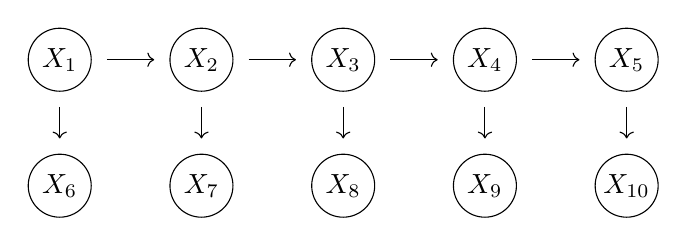
\begin{tikzpicture}[scale=2.0]
    \draw (0,0) circle (0.2) node[] {$X_1$};
    \draw[->] (0.3,0.0) -- (0.6,0.0);
    \draw (0.9,0) circle (0.2) node[] {$X_2$};
    \draw[->] (1.2,0.0) -- (1.5,0.0);
    \draw (1.8,0) circle (0.2) node[] {$X_3$};
    \draw[->] (2.1,0.0) -- (2.4,0.0);
    \draw (2.7,0) circle (0.2) node[] {$X_4$};
    \draw[->] (3.0,0.0) -- (3.3,0.0);
    \draw (3.6,0) circle (0.2) node[] {$X_5$};

    \draw[->] (0.0,-0.3) -- (0.0,-0.5);
    \draw (0.0,-0.8) circle (0.2) node[] {$X_6$};
    \draw[->] (0.9,-0.3) -- (0.9,-0.5);
    \draw (0.9,-0.8) circle (0.2) node[] {$X_7$};
    \draw[->] (1.8,-0.3) -- (1.8,-0.5);
    \draw (1.8,-0.8) circle (0.2) node[] {$X_8$};
    \draw[->] (2.7,-0.3) -- (2.7,-0.5);
    \draw (2.7,-0.8) circle (0.2) node[] {$X_9$};
    \draw[->] (3.6,-0.3) -- (3.6,-0.5);
    \draw (3.6,-0.8) circle (0.2) node[] {$X_{10}$};
    \end{tikzpicture}
\end{figure}
\begin{subproblem}{1}
Write down a full factorization of $p(X_{1:10})$ implied by the graphical model. Your factorization should be as simple as possible (\textit{simplicity is measured by the number of $X_\star$ terms that show up in your final expression}).
\end{subproblem}

\begin{subproblem}{1}
What is the Markov boundary of $X_4$?
\end{subproblem}


\begin{subproblem}{1}
What is the Markov boundary of $X_8$?
\end{subproblem}

\begin{subproblem}{2}
Write down a full factorization of $p(X_{1:3},X_{5:10}|X_4)$ that is as simple as possible.
\end{subproblem}

\end{problem}

\begin{problem}{13}
    Consider the two following MA(4) processes:
    \begin{align}
        X_t &= W_t + \theta_3 W_{t-3} + \theta_4 W_{t-4} + \theta_c \\
        Y_t &= W_t + \theta_1 W_{t-1} + \theta_4 W_{t-4},
    \end{align}
    where $W_t$ is drawn from $\mathcal{N}(0, \sigma_W^2)$ and all the $\theta_\star$ are constants.
    \begin{subproblem}{2}
        What is the mean, $\mu_X(t)$, of the $\{X_t\}$ process? Justify your answer.
    \end{subproblem}

    \begin{subproblem}{3}
        What is the covariance, $\gamma_X(t,s)$, of the $\{X_t\}$ process?
    \end{subproblem}
    
    \begin{subproblem}{1}
        Is $\{X_t\}$ drawn from a weakly stationary process?
    \end{subproblem}
    \begin{subproblem}{5}
        What is the cross-covariance, $\gamma_{X,Y}(t,s)$, between $X_t$ and $Y_s$?
    \end{subproblem}
    \begin{subproblem}{2}
       Is it possible for $\gamma_{X}(t,t) = 0$? If so, what is one value of $\theta_1, \theta_2, \theta_3, \theta_4$ that satisfied this? Limit yourself to the real numbers.
    \end{subproblem}
\end{problem}

\begin{problem}{10}
    Consider the following two models:
    \begin{align}
        X_t &= 2.5X_{t-1} - X_{t-2} + W_t - 2 W_{t-1} \\
        Y_t &= 0.7Y_{t-1} + 0.3Y_{t-2} + W_t - 0.4 W_{t-1},
    \end{align}
    where $W_t$ is drawn from $\mathcal{N}(0, \sigma_W^2)$.
    \begin{subproblem}{3}
        Identify $\{X_t\}$ as ARMA$(p,q)$. \textit{Watch out for parameter redundancy.}
    \end{subproblem}
    \begin{subproblem}{1}
        Is $\{X_t\}$ causal? Justify your answer.
    \end{subproblem}
    \begin{subproblem}{1}
        Is $\{X_t\}$ invertible? Justify your answer.
    \end{subproblem}
    \begin{subproblem}{3}
        Identify $\{Y_t\}$ as ARMA$(p,q)$.
    \end{subproblem}
    \begin{subproblem}{1}
        Is $\{Y_t\}$ causal? Justify your answer.
    \end{subproblem}
    \begin{subproblem}{1}
        Is $\{Y_t\}$ invertible? Justify your answer.
    \end{subproblem}
\end{problem}

\begin{problem}{7}
    Consider an AR$(2)$ process with the equations:
    \begin{align}
        P(B) = (1-0.4B)(1+0.4B).
    \end{align}
    Please answer the following questions:
    \begin{subproblem}{1}
        Is the process causal? 
    \end{subproblem}
    \begin{subproblem}{6}
        What is the correlation function $\rho(t,t+h)=\rho(h)$? \textit{Hint: remember that $\rho(0) = 1$.}
    \end{subproblem}
\end{problem}

\end{document}
